\documentclass[12pt]{article}

\usepackage{sbc-template}

\usepackage{graphicx,url}

\usepackage{amsmath}

\usepackage[dvipsnames]{xcolor}

\usepackage[brazil]{babel}   
%\usepackage[latin1]{inputenc}  
\usepackage[utf8]{inputenc}  
% UTF-8 encoding is recommended by ShareLaTex
% o comando abaixo permite que a saida no PDF possa ser copiada com acentos corretamente para outro documento
\usepackage[T1]{fontenc}

     
\sloppy

\title{Predição de cobertura florestal usando árvores de decisão no Apache Spark}

\author{João Ferreira\inst{1}, Rodrigo Tavares\inst{1}, Eduardo Ogasawara\inst{1} }


\address{Programa de Pós-graduação em Ciência da Computação\\ 
Centro Federal de Educação Tecnológica Celso Suckow da Fonseca (CEFET/RJ)\\
  Caixa Postal 20.271-110 -- Rio de Janeiro -- RJ -- Brasil
  \email{rtavaresrj87@gmail.com, joao.parana@gmail.com,
  eogasawara@ieee.org}
}

\begin{document} 

\maketitle

\begin{abstract}
Forests are an important part of the planet's ecosystem and discovering forest cover forecasting techniques can help conservation agencies at work to maintain and even improve the quality of forests. This work uses Decision Tree and Random Forests algorithms on a set of soil information data for forest cover evaluation and forecasting. The algorithms were executed using Apache Spark, to compare their execution in serialized and parallelized versions. Different numbers of cores were used, evaluating the elapsed-time, speed-up and efficiency, in order to evaluate the advantages of the parallelized execution of algorithms
\end{abstract}
     
\begin{resumo} 
As florestas são parte importante do ecosistema do planeta e descobrir técnicas de previsão de cobertura florestal pode ajudar as agências de preservação no trabalho de manter e até melhorar a qualidade das florestas. Este trabalho utiliza os algoritmos {\it Decision Tree} e {\it Random Forests} sobre um conjunto de dados de informações sobre solo, para avaliação e previsão de cobertura florestal. Os algoritmos foram executados com Apache Spark, para comparar a execução dos mesmos em versões serializadas e paralelizadas. Foram utilizados diferentes números de núcleos de processador, aferindo o {\it elapsed-time}, {\it speed-up} e eficiência, de modo a avaliar as vantagens da execução paralelizada dos algoritmos.
\end{resumo}


\section{Introdução}

As florestas possuem grande importância para a preservação da vida no planeta, uma vez que elas renovam o oxigênio, equilibram o sistema climático, protegem o solo e alimentam um variado ecossistema. As alterações na cobertura florestal desestruturam o sistema ecológico e ameaçam a vida no planeta. A ocorrência de desmatamento, por exemplo, pode causar uma diminuição na capacidade da floresta em absorver o carbono da atmosfera, além de permitir a elevação da temperatura do solo piorando a sua qualidade. 

Para o acompanhamento, mapeamento da cobertura florestal e uso da terra, pode-se usar técnicas de mineração de dados, particularmente as ferramentas de classificação (aprendizado de máquina do tipo supervisionando).  Dentre estas ferramentas, destaca-se a árvore de decisão ({\it Decision Tree}) que permite prever, por exemplo, quais partes da terra são boas para cultivar uma dada vegetação quando é conhecida a localização e propriedades químicas do solo.

A popularidade da árvore de decisão vem do fato de permitir fazer classificação (predizer valores discretos chamados classes), regressão (predizer valores contínuos), estimativa de probabilidade e agrupamentos ({\it clustering}). Além disso o resultado é facilmente interpretado.
Outras vantagens incluem:  i) os dados não precisam ser normalizados e aceitam valores em escalas distintas; ii) São robustas, ou seja, não sofrem efeitos de valores extremos ({\it outliers}); iii) são paralelizáveis em ambiente de computação de alto desempenho; iv) consomem dados de tipos diferentes. Por tudo isso, é bastante utilizada na prática, em particular quando são organizadas em conjuntos de árvores como no caso do algoritmo chamado {\it Random Forests} que permite combinar várias árvores de decisão na análise de um {\it dataset} (conjunto de dados de entrada).

As árvores de decisão se comportam como uma função de predição no contexto de aprendizado supervisionado e funcionam da seguinte forma:
\begin{itemize}
\item Existe um dado conjunto de registros de entrada ({\it dataset}) onde cada tupla contém um vetor de N atributos (também chamado {\it features}) sendo um deles um valor de saída (também chamado {\it target} ou predição)

\item O dataset pode ser dividido em três partições (treinamento, validação e teste)

\item O algoritmo executado sobre a parte do dataset relativo a treinamento consegue criar a árvore de decisão.

\item Executando o algoritmo de árvore de decisão sobre o dataset de validação (também chamado validação cruzada) permite ajustar os hiperparâmetros (tais como profundidade máxima da árvore, quantidade de atributos a considerar, bin-count\footnote{bin-count é o número que define a quantidade de agrupamentos a ser feito em um dado atributo para convertê-lo em categorias diminuindo a dimensionalidade.}). Em geral, o processamento do dataset de validação tende a criar um modelo enviesado (biased)

\item Finalmente, executando o algoritmo sobre o dataset de teste é possível avaliar os indicadores de acurácia para verificar se o algoritmo poderá ser usado em outros dados que não façam parte do dataset original, ou seja, se fará a predição correta de novos dados obtidos no mundo real. O processamento do dataset de teste permite criar um modelo não-enviesado ({\it unbiased})
\end{itemize}
O processo descrito acima é típico em aprendizado de máquina supervisionado e o que muda entre as diversas execuções são o algoritmo e seus hiperparâmetros, pois para um problema em particular é possível encontrar uma configuração que se adeque melhor e dê resultados superiores em termos de acurácia e/ou eficiência.

\begin{figure}[!ht]
	\centering
	\begin{minipage}[t]{0.35\textwidth}
        % 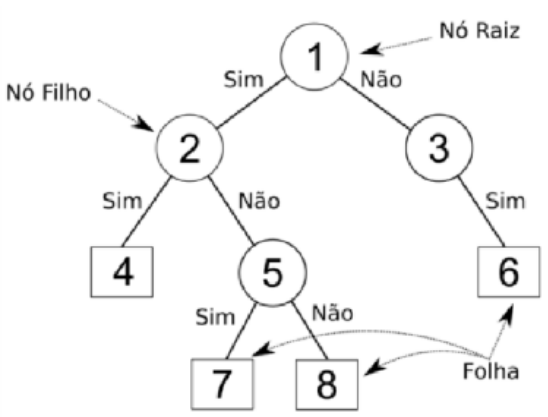
\includegraphics[width=300,height=200]{img/arvore.png}
        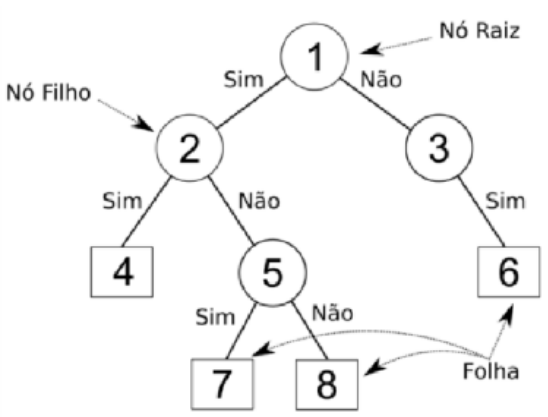
\includegraphics[width=\textwidth]{img/arvore.png}
        \centering
	\end{minipage}
	\caption
	{
	    Estrutura geral de uma árvore de decisão.
	}
	\label{fig:arvore}
\end{figure}

Para obter uma intuição sobre este processo pode-se detalhar a estrutura da árvore de decisão e as características do schema do dataset sob estudo.  

A árvore de decisão possui uma estrutura simples, como pode ser visto na figura \ref{fig:arvore}.  Os Nós 1, 2, 3 e 5 representam predicados sobre os atributos (também chamados \emph{features} na nomenclatura de aprendizado de máquina). Os predicados são coisas do tipo: \emph{Horizontal Distance To Hydrology between 50 and 100, Soil type equals "Granile", Elevation between 100 and 200}, etc.
Os Nós 4, 6, 7 e 8 são folhas e nos levam a uma decisão como valor de saída. Um exemplo dessa saída poderia ser, no nosso caso: \emph{ponderosa pine} ou \emph{Cottonwood/Willow}, já que os 7 tipos de cobertura vegetal no \emph{dataset} sob estudo são:
\emph{1 - Spruce/Fir ; 2 - Lodgepole Pine  ; 3 - Ponderosa Pine  ; 4 - Cottonwood/Willow  ; 5 - Aspen  ;   6 - Douglas-fir  ;  7 - Krummholz}.

O \emph{dataset} utilizado no experimento foi obtido em \emph{https://www.kaggle.com}  postado por \emph{UCI Machine Learning} da Universidade da Califórnia no endereço \emph{uciml/forest-cover-type-dataset:
https://www.kaggle.com/uciml/forest-cover-type-dataset}. Este \emph{dataset} será detalhado nas seções Avaliação experimental e Metodologia.  Na figura \ref{fig:vegetacao} podem ser vistos alguns tipos de cobertura vegetal, típicas da região em estudo.

\begin{figure}[!ht]
	\centering
	\begin{minipage}[t]{0.55\textwidth}
        % 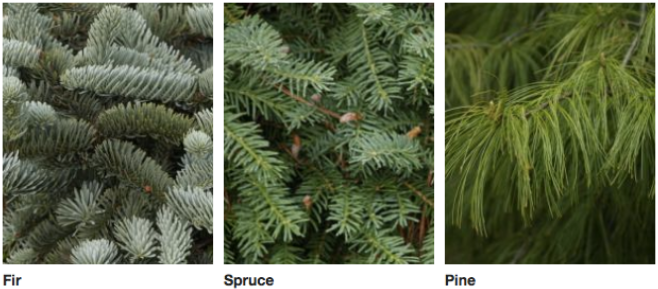
\includegraphics[height=180]{img/vegetacao.png}
        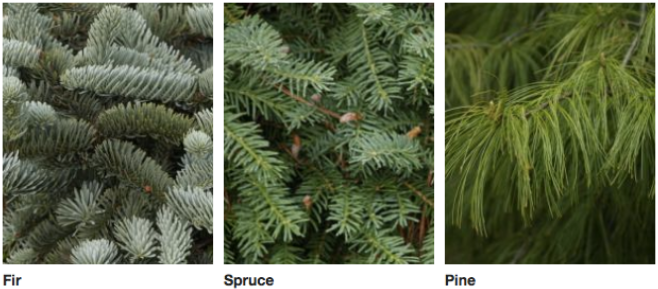
\includegraphics[width=\textwidth]{img/vegetacao.png}
        \centering
	\end{minipage}
	\caption
	{
	    Três tipos de cobertura vegetal das observadas nas florestas do Colorado (USA).
	}
	\label{fig:vegetacao}
\end{figure}

Definida a estrutura de dados da árvore de decisão é preciso descrever o comportamento dinâmico do processo de aprendizado. O funcionamento do algoritmo se dá pela divisão do conjunto de dados em subconjuntos, de forma recursiva. A árvore de decisão é formada por nós e a medida que os dados de entrada são lidos, os nós são adicionados usando um algoritmo de análise de entropia. Este algoritmo é executado para que a árvore represente da melhor forma possível a distribuição estatística dos dados, evitando modelos enviesados e incorretos.  

Observe que, quando se caminha pela árvore criada, percorrendo em profundidade da raiz até uma dada folha, passando pelas avaliações dos predicados, encontra-se as razões pelas quais chega-se a um dado valor de saída definido na folha e a árvore é facilmente interpretada do ponto de vista semântico.

Esta monografia está organizada da seguinte forma: na seção 2 apresenta-se uma revisão bibliográfica sobre os dois aspectos do trabalho que são árvores de decisão e Apache Spark; na seção 3 descreve-se a metodologia usada no trabalho para mostrar a validade da hipótese de usar aprendizado de máquina para predição de cobertura florestal no Apache Spark com acurácia desejada; na seção 4 faz-se uma breve exposição dos trabalhos relacionados ao tema ; na seção 5 apresenta-se os resultados de uma avaliação experimental focada na avaliação do desempenho do sistema de processamento distribuído, com particionamento horizontal dos dados para processar grandes volumes usando 2 algoritmos de aprendizado de máquina, neste caso {\it Decision Trees} e {\it Random Forests}; na seção 6 apresenta-se as considerações finais e as direções para futuros trabalhos de pesquisa relacionados a este trabalho.

\section{Revisão bibliográfica} 
\label{sec:Revisão bibliográfica}

Tarefas de predição com aprendizagem supervisionada cpmpõem um campo bem estudado em Aprendizagem de Máquinas, com muitas formulações diferentes onde é possível citar \cite{settles2010active} que também destaca técnicas de aprendizado semi-supervisionado.  Existem muitos algoritmos que podem ser usados para resolver este problema, desde regressão linear simples até redes neurais, passando por árvores de decisão (\emph{Decision Trees}) e máquinas de vetor de suporte. \emph{Decision Trees} e \emph{Randon Forests} estão na categoria de Aprendizado Simbólico que é um  \emph{framework} unificado para resolução de uma ampla gama de problemas incluindo classificação, regressão, estimativa de densidade, e até mesmo aprendizado semi-supervisionado (não tratado neste trabalho), como dito em \cite{criminisi2012decision}.  

Segundo \cite{breiman2001random} as \emph{Randon Forests} são uma combinação de preditores de árvores (\emph{Decision tree}), de modo que cada árvore depende dos valores de um vetor aleatório amostrado independentemente e com a mesma distribuição para todas as árvores na floresta. O erro de generalização para as florestas converge à medida que o número de árvores na floresta se torna grande. A intuição por trás da proposta é que com várias árvores o sobre-ajuste (\emph{overfitting}) será minimizado permitindo uma melhor eficiência na predição correta da classificação. \cite{breiman2001random} observou também que Randon Forests podem ser aplicadas às tarefas de regressão onde a predição objetiva valores contínuos.

Dado que escolheu-se os métodos \emph{Decision Trees} e \emph{Randon Forests}  como os mais adequados passa-se a revisão sobre o Apache Spark que permite executar o algoritmo para um conjunto de dados extremamente grande. 

Em 2012 Matei Zaharia e seus colegas da UC Berkley publicaram um artigo \cite{Zaharia2012RDD} onde apresentaram uma nova abstração chamada \emph{Resilient Distributed Datasets} (RDD). Foi o início de uma nova solução de processamento de dados que abordou alguns dos pontos problemáticos do modelo \emph{MapReduce} usado, até então, no Apache Hadoop e similares. Os RDDs podem ser armazenados em cache na memória, o que é uma grande vantagem para algoritmos iterativos. Além disso o RDD usa estratégias de implementação que permitem uma melhor tolerância a falhas e melhorias de desempenho por considerar a localidade dos dados. A API para RDDs é segura por tipo (\emph{type-safe}) e neste sentido é semelhante a outras soluções tal como o Scalding do Twitter. No RDD as transformações são de avaliação tardia e retornam RDDs \emph{well-typed} (tipagem forte) e são definidas usando funções regulares do Scala. As ações são o mecanismos do framework para materializar o resultado de um dado processamento.

Após o sucesso do RDD a  comunidade Spark introduziu uma API denominada \emph{Dataframe} e um novo mecanismo de execução baseado no SQL para apoiá-la como pode ser visto em \cite{armbrust2015spark}. Neste trabalho os autores abordaram algumas das limitações de otimização de RDDs e usaram técnicas de otimização de última geração através do otimizador Spark SQL Catalyst\footnote{Catalyst é o subprojeto do Spark com foco em otimização lógica e baseada em custo.}, aliado a geração de código em tempo de execução usando o Tungsten\footnote{Tungsten é o subprojeto do Spark com foco em geração de byte-code para a JVM em tempo de execução para traduzir os escalonamentos calculados e otimizados pelo Catalyst em código binário da JVM. As transformações de avaliação tardia precisam desta funcionalidade para prover ajuste dinâmico.}. A API \emph{Dataframe} sofre por falta de segurança de tipo e então foi desenvolvido também uma API de tipagem mais forte, chamada \emph{Dataset} que permite o uso de Schemas fortemente tipados na interface SQL fornecendo ao Catalyst subsídios para produzir otimizações ainda melhores que consideram informações de tipo de dado como elementos para heurísticas mais elaboradas.   

Sobre a API  Dataset foi possível desenvolver uma plataforma para Aprendizado de Máquina a qual deram o nome de MLLib. Esta API foi apresentada em \cite{meng2016MLlib} e foram implementados diversos algoritmos de Aprendizado de Máquina paralelizáveis onde os dados podem ser particionados horizontalmente e distribuídos entre diversas máquinas do Cluster e executados transparentemente via Spark. A implementação DecisionTreeModel e RandomForest são as utilizadas neste trabalho para predição de cobertura florestal.


\begin{figure}[!ht]
	\centering
	\begin{minipage}[t]{0.55\textwidth}
        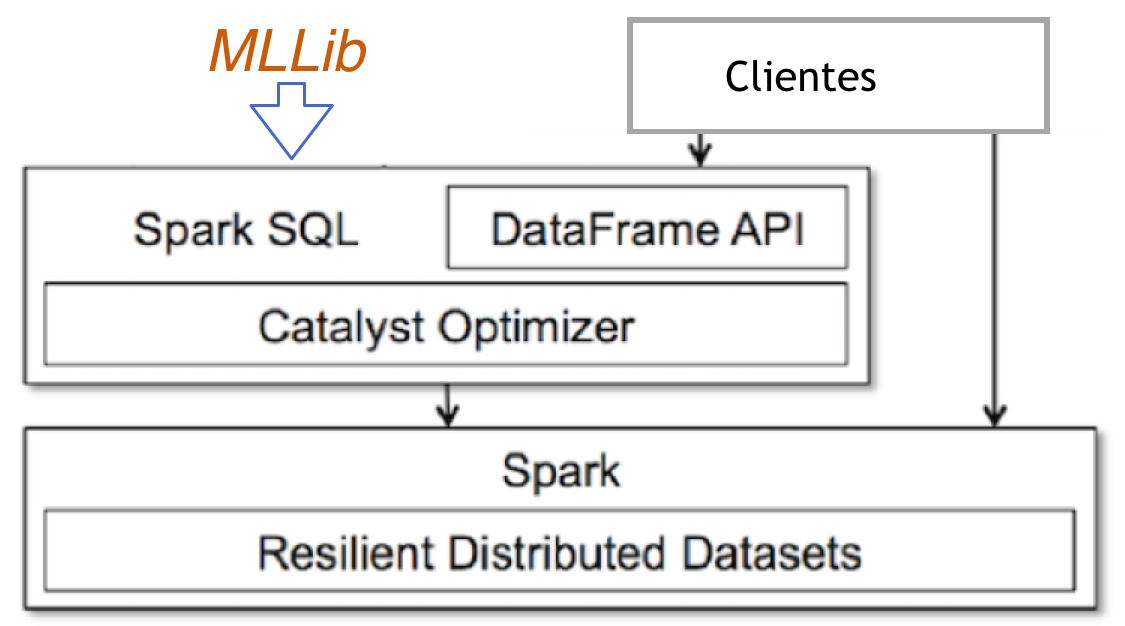
\includegraphics[width=\textwidth]{img/arq-spark.png}
        \centering
	\end{minipage}
	\caption
	{
	   Arquitetura Spark.
	}
	\label{fig:arqspark}
\end{figure}


A figura \ref{fig:arqspark} mostra os componentes do Spark e como estão relacionados. A MLLib interage com a API de DataFrame que por sua vez usa as funcionalidades do Catalyst para otimizar o código gerado. Este código usa a API RDD que provê a resiliência em ambiente distribuído.

\section{Metodologia}
\label{sec:Metodologia}

Para o treinamento da Árvore de Decisão foi utilizado o \emph{dataset} covtypeData \footnote{link para a descrição completa: https://www.kaggle.com/uciml/forest-cover-type-dataset}. Este dataset possui 581.012 medidas de variáveis cartográficas sobre a cobertura vegetal numa dada região. As colunas são: i) Elevation: elevação em metros ; ii) Aspect: aspecto em graus azimute ; iii) Slope: inclinação em graus ; iv) Horizontal Distance To Hydrology: distância horizontal até fonte de água ; v) Vertical Distance To Hydrology: distância vertical até fonte de água; vi) Horizontal Distance To Roadways: distância horizontal até a estrada mais próxima ; vii) Hillshade 9am (0 to 255 index): Índice de sombra da colina às 9h, solstício de verão ; viii) Hillshade Noon (0 to 255 index): Índice de sombra da colina ao meio dia, solstício de verão ; ix) Hillshade 3pm (0 to 255 index): Idem para 3 da tarde ; x) Horizontal Distance To Fire Points: distância horizontal até os pontos de ignição de incêndios mais próximos ; xi) Wilderness Area (4 binary columns, 0 = absence or 1 = presence): Designação para o quanto uma área é de região selvagem ; xii) Soil Type (40 binary columns, 0 = absence or 1 = presence): Designação para o tipo de solo ; xiii) Cover Type (7 types, integers 1 to 7): Designação do tipo de cobertura florestal. Esta última coluna é o que chamamos de target feature. 

Uma análise do Schema do \emph{dataset} revela que existem um total de 55 \emph{features} sendo que Wilderness Area e Soil Type foram codificadas no modo one-hot encoding \footnote{Uma codificação one-hot é um processo pelo qual as variáveis categóricas são convertidas em um conjunto de variáveis booleanas para serem fornecidas aos algoritmos de Machine Learning para obter predição de melhor qualidade não sofrendo influência da informação de ordenação intrínseca aos valores contínuos originais.} com semântica booleana. 

\begin{figure}[!ht]
	\centering
	\begin{minipage}[t]{0.95\textwidth}
        % 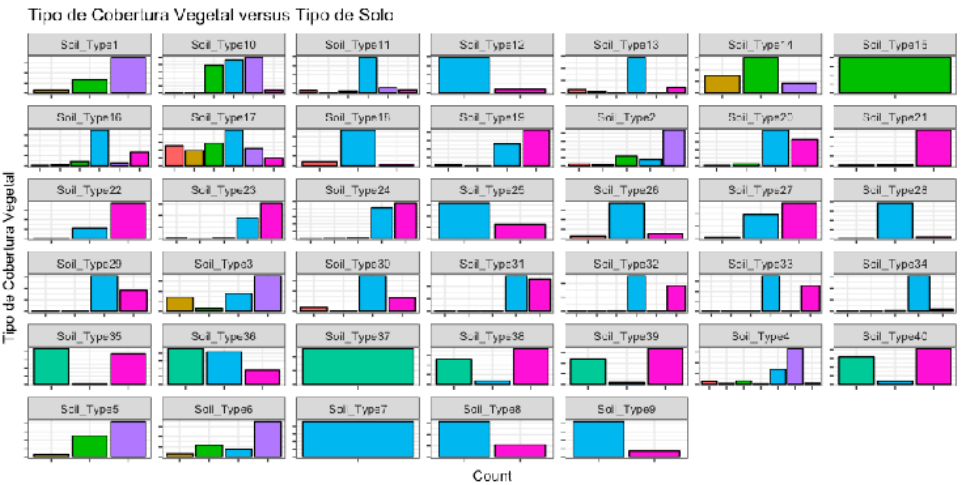
\includegraphics[height=280,width=400]{img/cobertura_x_solo.png}
        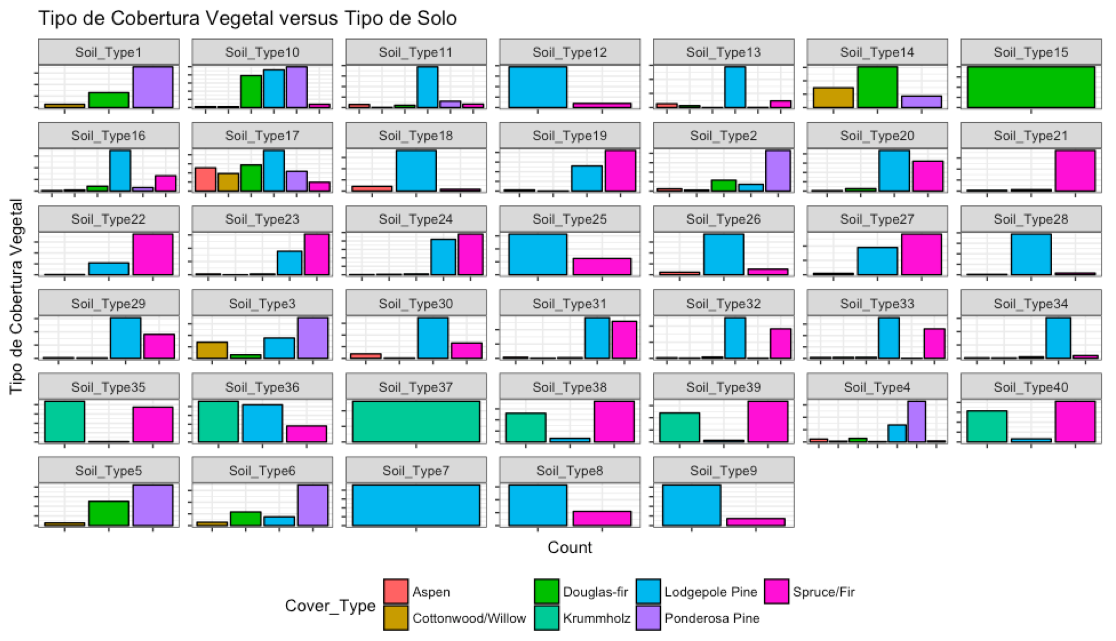
\includegraphics[width=\textwidth]{img/cover-x-soiltype.png}
        \centering
	\end{minipage}
	\caption
	{
	    Tipo de Cobertura Vegetal versus Tipo de Solo.
	}
	\label{fig:vegetalxsolo}
\end{figure}

Uma análise exploratória dos dados, usando linguagem R, mostra uma forte dependência entre o tipo de solo e o tipo de cobertura florestal encontrada, como pode ser visto na figura 3 - Tipo de Cobertura Vegetal versus Tipo de Solo. Por exemplo, observa-se na figura que em 5 tipos de solo diferentes (15, 2, 28, 37, 7) predominam um único tipo de cobertura florestal enquanto que para o tipo de solo 17 há uma distribuição mais igualitária de espécies totalizando 6 espécies diferentes das 7 existentes (apenas a espécie Krummholz não é encontrada nesta área).

O modêlo (hipótese) é de que árvores de decisão são uma boa opção para prever como fica a cobertura florestal dado um conjunto de dados cartográficos. A implementação escolhida para árvore de decisão foi a fornecida pelo Apache Spark pois permite a paralelização do algoritmo além de fornecer opção para uso de \emph{Random Forests} que são uma generalização de árvores de decisão e permitem obter uma acurácia maior manipulando um conjunto composto por várias árvores de decisão para um mesmo conjunto de dados.

\section{Trabalhos relacionados}
\label{sec:Trabalhos relacionados}

No dataset de cobertura florestal, que foi objeto de estudo deste trabalho, existe uma relação de 120 para 1 entre a cardinalidade de uma das classes de cobertura vegetal comparada com outra. Isto é conhecido como desequilíbrio de classe (imbalanced) e foi objeto de estudo de \cite{del2014use} no artigo \emph{On the use of MapReduce for imbalanced big data using Random Forest} que estuda o problema de desempenho dos algoritmos de aprendizado de máquina quando existe desequilíbrio de classe, ou seja, quando existem poucas amostras no dataset para algumas das classes existentes em comparação com as outras. Os autores analisam o desempenho de várias técnicas utilizadas para lidar com desequilíbrio no conjuntos de dados no cenário de bigdata usando o classificador Random Forest como \emph{baseline}. O classificador \emph{Random Forest} foi escolhido pelos autores pois fornece uma base sólida para a comparação devido ao seu desempenho, robustez e versatilidade.

Em \cite{cutler2007random}  - Random Forests for Classification in Ecology  os autores listam diversas vantagens do classificador Random Forests em comparação a outros métodos nas pesquisas de ecologia : \emph{i)} alta precisão (acurácia) na classificação; \emph{ii)} um novo método para determinar a importância variável; \emph{iii)} capacidade de modelar interações complexas entre variáveis preditoras; \emph{iv)} flexibilidade para realizar vários tipos de análise de dados estatísticos, incluindo regressão, classificação e aprendizado não-supervisionado; e \emph{v)} um algoritmo para imputar dados ausentes. Os autores comparam as acurácias obtidas entre Random Forests e outros quatro classificadores estatísticos comumente usados na Ecologia e observaram alta precisão do método Random Forests em todas as aplicações de classificação avaliadas.

Em \cite{rodriguez2012assessment} - An assessment of the effectiveness of a random forest classifier for land-cover classification] mencionam que o monitoramento da cobertura do solo usando dados de detecção remota requer métodos de classificação robustos e estudam a validade do uso do classificador Random Forests. A conclusão é que este método apresenta ótimos resultados com o dataset \emph{Landsat 4-5 Thematic Mapper} \footnote{Detalhes sobre as imagens de satélite podem ser obtidas em https://lta.cr.usgs.gov/TM} utilizado. 

\section{Avaliação experimental}
\label{sec:Avaliação experimental}

Na avaliação experimental criamos um dataset mínimo com apenas 2999 tuplas para realizar uma análise exploratória preliminar para efeito didático de entendimento da implementação do Spark.

Quanto ao dataset, houve a necessidade de alguns ajustes na versão original que foi transformada para um Schema como este abaixo:

\begin{verbatim}
 |-- Elevation: integer
 |-- Aspect: integer
 |-- Slope: integer
 |-- Horizontal\_Distance\_To\_Hydrology: integer
 |-- Vertical\_Distance\_To\_Hydrology: integer
 |-- Horizontal\_Distance\_To\_Roadways: integer
 |-- Hillshade\_9am: integer
 |-- Hillshade\_Noon: integer
 |-- Hillshade\_3pm: integer
 |-- Horizontal\_Distance\_To\_Fire\_Points: integer
 |-- Wilderness\_Area\_0: integer - boolean semantics
 |-- Wilderness\_Area\_1: integer - boolean semantics
 |-- Wilderness\_Area\_2: integer - boolean semantics
 |-- Wilderness\_Area\_3: integer - boolean semantics
 |-- Soil\_Type\_0: integer
 |-- Soil\_Type\_1: integer
. . . 
 |-- Soil\_Type\_38: integer
 |-- Soil\_Type\_39: integer
 |-- Cover\_Type: double
\end{verbatim}

As features Wilderness\_Area e Soil\_Type foram codificadas no modo \emph{one-hot encoding} que é mais adequada para a implementação da Árvore de Decisão pois são atributos categóricos e nesta codificação perdem a informação de ordenação melhorando o desempenho do algoritmo eliminando este viés. O total de features são: 10 com valores inteiros, 44 são categóricas e uma é \emph{target} e neste caso ponto flutuante mas com semântica de inteiro variando de 1 a 7.

Um exemplo de segmento de Árvore de Decisão encontrada com profundidade limitada a 5 é mostrada abaixo para efeito ilustrativo.

\begin{verbatim} 

DecisionTreeClassificationModel of depth 5 with 63 nodes
  If (feature 13 <= 0.0)
   If (feature 5 <= 800.0)
    If (feature 8 <= 103.0)
     If (feature 0 <= 2880.0)
      If (feature 0 <= 2606.0)
       Predict: 2.0
      Else (feature 0 > 2606.0)
       Predict: 5.0
     Else (feature 0 > 2880.0)
      If (feature 1 <= 88.0)
       Predict: 2.0
      Else (feature 1 > 88.0)
       Predict: 5.0
    . . .    
\end{verbatim} 

%
%\begin{figure}[!ht]
%	\centering
%	\begin{minipage}[t]{0.999\textwidth}
%        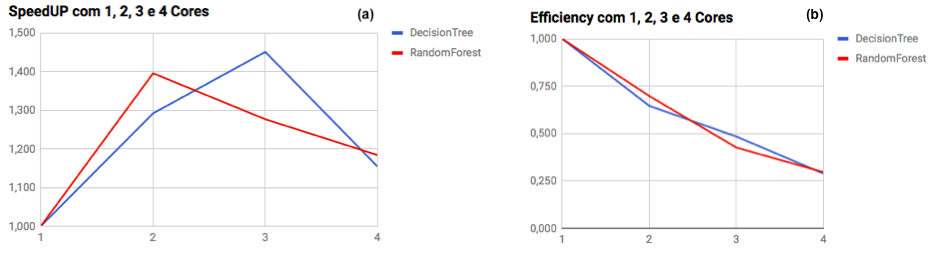
\includegraphics[width=\textwidth]{img/only-graph.png}
%        \centering
%	\end{minipage}
%	\caption
%	{
%	   (a) Speed-up  (b) Eficiência
%	}
%	\label{fig:speedup}
%\end{figure}

Quanto a tomada de medidas usamos as 3 métricas seguintes: Tempo Decorrido (elapsed-time), Speed-up e Eficiência. A métrica mais importante é a de Tempo Decorrido (elapsed-time) pois serve para calcular todas as outras. Considere o  exemplo de um sistema computacional S1 com 8 processadores. Pode-se executar um dado processo usando apenas um processador, e depois 2, 3, 4, 5, 6, 7 e por ultimo 8. Teremos ao final um conjunto de medidas de tempo decorrido: T1, T2, ... Tp , com p == 8.

% $\textbf{elaspsed\_time} \rightarrow\quad T_1, T_2, T_3, T_4, T_5, T_6, ... T_p$

\[
    \textbf{elaspsed\_time} \rightarrow\quad T_1, T_2, T_3, T_4, T_5, T_6, ... T_p
\]

Em seguida pode-se calcular o Speed-up, ou seja, medir o quanto efetivo que está sendo o usado pelos processadores para resolver o meu problema de modo paralelizado

\[
    \textbf{speed\_up} \rightarrow\quad S_{up} = \frac{T_1}{T_p}
\]

Por último pode-se calcular a eficiência. A eficiência $\xi$ é definida como a razão entre o speed-up e a quantidade de processadores. Eficiência perto de 1 significa que os processadores estão sendo usado eficientemente

\[
    \textbf{efficiency} \rightarrow\quad \xi = \frac{S_{up}}{p}
\]

A figura \ref{fig:experimentdata} apresenta a tabela com os resultados das medidas de elaspsed\_time, speed\_up e eficiência inferidos na realização do experimento:

%\begin{minipage}[t]{0.55\textwidth}
        %\includegraphics[width=\textwidth]

\begin{figure}[!ht]
	\centering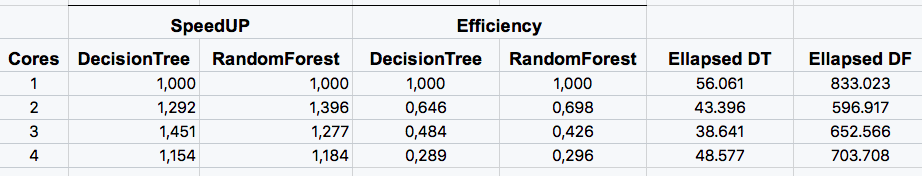
\includegraphics[width=\linewidth]{img/experiment-data.png}
	\caption{Dados experimentais coletados.}
	\label{fig:experimentdata}
\end{figure}

O gráfico da figura \ref{fig:speedup} mostra a evolução do speed\_up utilizando 1, 2, 3 e 4 Cores:

\begin{figure}[!ht]
	\centering
	\begin{minipage}[t]{0.55\textwidth}
        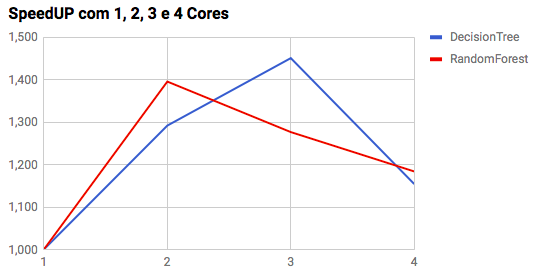
\includegraphics[width=\textwidth]{img/speed-up.png}
        \centering
	\end{minipage}
	\caption
	{
	   Speed-up.
	}
	\label{fig:speedup}
\end{figure}

O gráfico da figura \ref{fig:efficiency} mostra a evolução da eficiência utilizando 1, 2, 3 e 4 Cores:

\begin{figure}[!ht]
	\centering
	\begin{minipage}[t]{0.55\textwidth}
        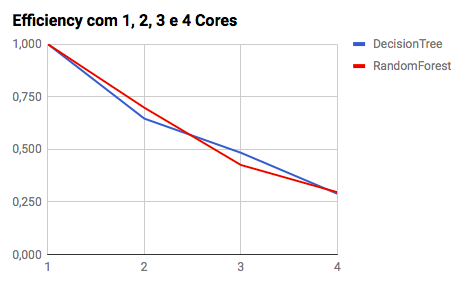
\includegraphics[width=\textwidth]{img/efficiency.png}
        \centering
	\end{minipage}
	\caption
	{
	   Eficiência.
	}
	\label{fig:efficiency}
\end{figure}

O comportamento observado com mais de três cores (4 neste exemplo) pode parecer anômalo, porém é natural caso se considere o fato de que um dos Cores é usado pelo Driver do Spark e portanto dificulta o trabalho do Worker que roda neste mesmo Core.

A seguir nas figuras \ref{fig:scala-code} e \ref{fig:predict-scala-code} ilustra-se o código Scala usado para, respectivamente, treinar o modelo e fazer predição.


\begin{figure}[!ht]
	\centering
	\begin{minipage}[t]{0.55\textwidth}
        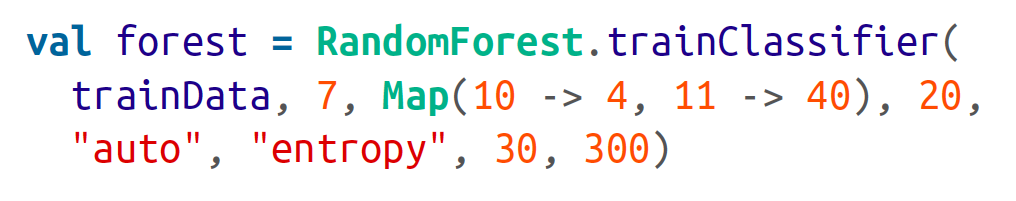
\includegraphics[width=\textwidth]{img/randomForest-Scala-code.png}
        \centering
	\end{minipage}
	\caption
	{
	   Código Scala que especifica o método de treinamento do classificador onde é informado os parâmetros de \emph{one-hot encoding, binning}, e os hiper-parâmetros.
	}
	\label{fig:scala-code}
\end{figure}


\begin{figure}[!ht]
	\centering
	\begin{minipage}[t]{0.55\textwidth}
        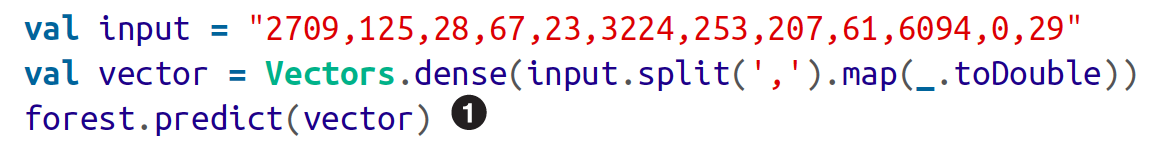
\includegraphics[width=\textwidth]{img/randomForest-predict-Scala-code.png}
        \centering
	\end{minipage}
	\caption
	{
	   Passando um array de dados é possível predizer a cobertura vegetal mais adequada considerando o comportamento estatístico do dataset de origem.
	}
	\label{fig:predict-scala-code}
\end{figure}

% - - - - - - - - - - - - - - 
% \begin{figure}[!ht]
%   \centering
%   \begin{minipage}[t]{0.55\textwidth}
%         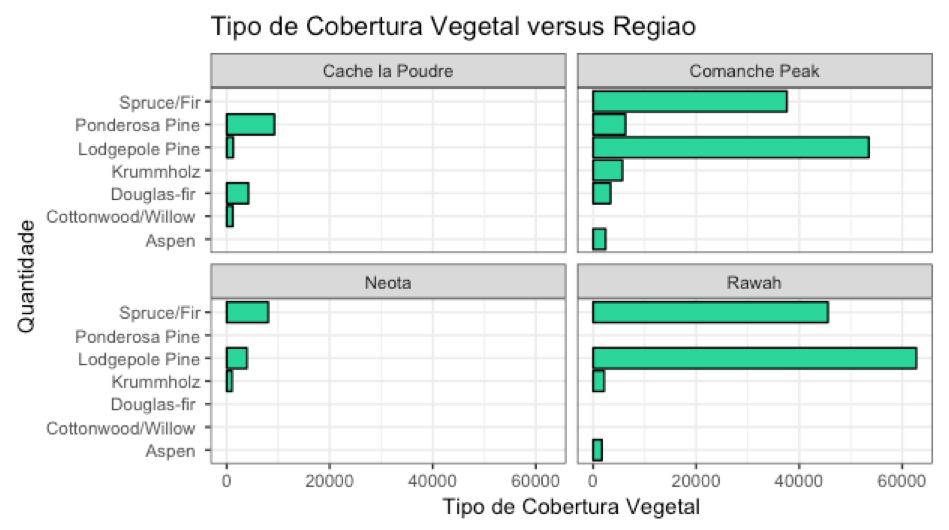
\includegraphics[width=\textwidth]{img/cover-x-region.png}
%         \centering
%   \end{minipage}
%   \caption
%   {
%      cover-x-region.
%   }
%   \label{fig:coverregion}
% \end{figure}
% 
% 
% 
% \begin{figure}[!ht]
%   \centering
%   \begin{minipage}[t]{0.55\textwidth}
%         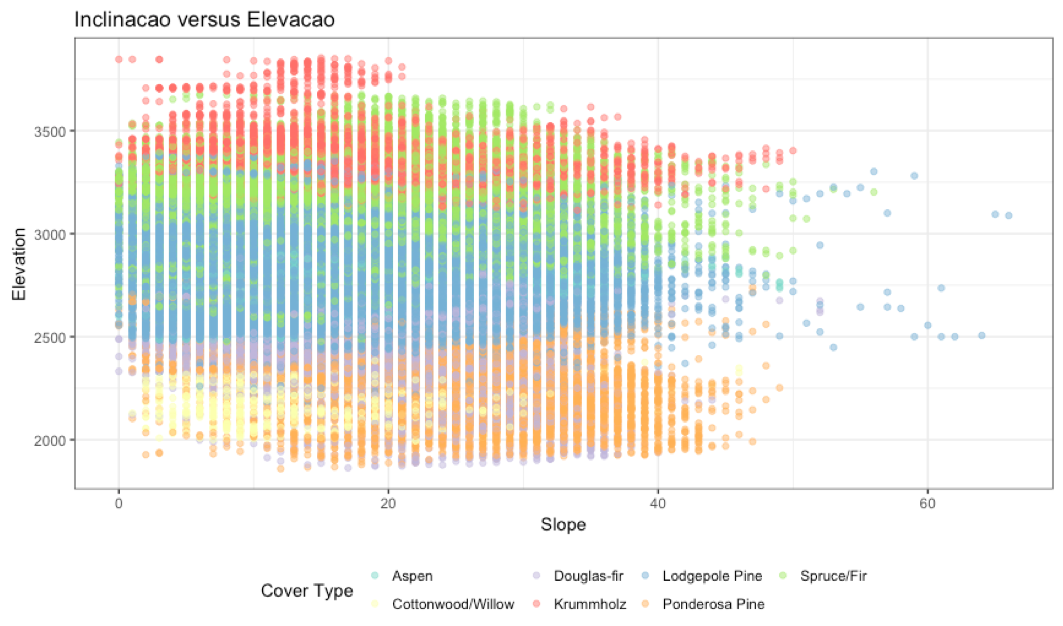
\includegraphics[width=\textwidth]{img/elevation-x-slope.png}
%         \centering
%   \end{minipage}
%   \caption
%   {
%      elevation-x-slope.
%   }
%   \label{fig:elevationslope}
% \end{figure}
% 

\section{Considerações finais}
\label{sec:Considerações finais}

É possível observar que os algoritmos {\it Decision Tree} e {\it Random Forests} apresentam boa capacidade de paralelização. A implementação com o Apache Spark utilizando o pacote MLlib se mostrou bastante objetiva e os resultados para as medidas de elapsed-time, speed-up e eficiência comprovam os benefícios da execução paralela destes algoritmos.

Trabalhos futuros podem avaliar o desempenho de Random Forests para Datasets ainda maiores, inclusive para temas diversos, como imputação de dados ausentes para valores numéricos e categóricos.

Existe também a oportunidade de executar o processo usando um Framework tal como o de \cite{ferreira2017} que poderá facilitar o trabalho de análise de resultados pois fornece mecanismo de execução de vários experimentos com coleta de proveniência e consolidação de resultados para análise posterior pelo cientista de dados. Neste contexto é possível experimentar outros algoritmos de aprendizado de máquina, com a capacidade de ajustar os hiper-parâmetros de forma declarativa em um workflow construído para este propósito.

\bibliographystyle{sbc}
\bibliography{sbc-template}

\end{document}
